\section{Test Methods}
There are a number of different types of tests appropriate for our project. The tests mentioned in this chapter are general tests that works equally well related to software development and hardware development. In Fig. \ref{fig:testing} a setup on how testing can be divided in to groups is displayed.

\begin{figure}[h]
    \centering
        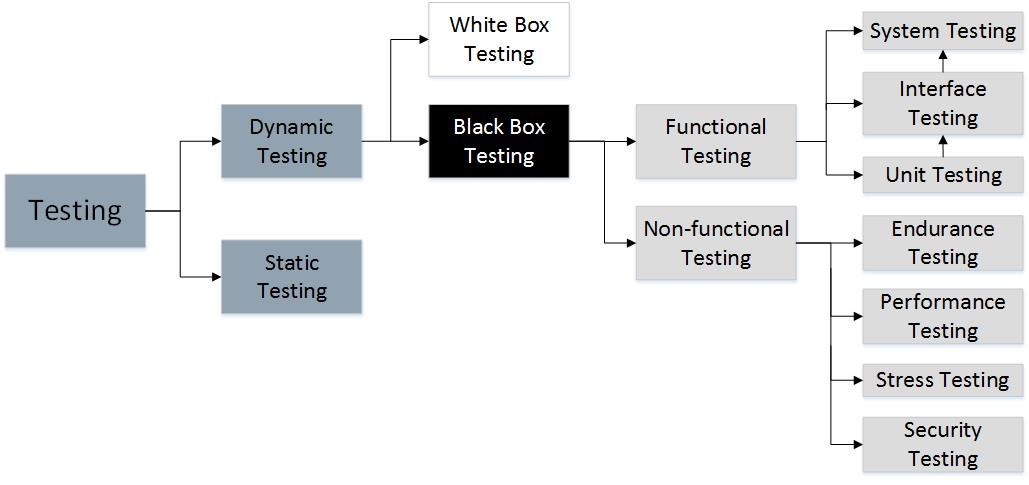
\includegraphics[width=0.9\textwidth]{VAPIQ-PICTURES/testing}
        \caption{Test Methods Diagram}
        \label{fig:testing}
\end{figure}

\subsection{Static Testing}
The primary purpose of Static Testing or Static Verification is to find errors in documentation and code. We do this through review, analysis, inspection, and walk-through. The purpose of this is to find deviations from the stakeholder needs. The results can be used to optimize development processes and provide input to dynamic testing \cite{ref3}. 

\subsection{Dynamic Testing}
Dynamic Testing can be conducted on the actual product. The purpose of this is to find deviations from expected values or the confirmed values \cite{ref3}. The main purpose of Dynamic Testing is to ensure consistency of the system.

\subsubsection{Black Box Testing}
In Black Box Testing the internal structure, design or code is not known to the tester. The main aspiration is to verify the functionality of the system under testing, and that it ensures traceability. 

\paragraph{Functional Testing} \\
Functional Testing is conducted to verify that the features developed for our systems are according to the functional Backlog Item. The tests are performed based on the Acceptance Criteria written by the Scrum Team or Tester. In Functional Testing, tests are performed by providing an input, verifying the output and comparing the actual results with the expected results.\\
\\
There are different levels of Functional Testing: 
\begin{itemize}
  \item Unit Testing - test to verify the smallest testable parts of a system. 
  \item Interface Testing - tests to evaluate whether systems or components pass data and control correctly to one another. To verify that all the interactions between these systems are working properly and errors are handled the right way. 
  \item System Testing - testing an integrated system to verify that it meets the specified requirements. 
\end{itemize}\\
\\
\paragraph{Non-Functional Testing} \\
Non-Functional Testing is a testing technique which does not focus on functional aspects of the system. It mainly focuses on the Non-Functional characteristics of the system such as performance, robustness and stability. Non-Functional Testing is performed at all test levels \cite{ref6}.\\
\\
There are different levels of Non-Functional Testing: 
\begin{itemize}
  \item Endurance Testing - Testing a system with a load extended over a period of time. This testing is performed to show how the system behaves under sustained use. 
  \item Performance Testing - Testing that is performed to determine how fast some aspect of a system performs under a particular workload. This test can for instance compare two systems to find out which performs better.
  \item Security Testing - Testing to check if the system is secure. This might be Information Security or Health, Safety amd Enviroment. 
  \item Stress Testing - Testing the system beyond normal operational capacity, often to a breaking point, in order to observe the results. Used to determine the capabilities of the system. 
\end{itemize}\\
\\
\subsubsection{White Box Testing}
White Box Testing is a method in which the internal structure or workings of a system is tested. In White Box Testing the internal structure or design being tested is known to the tester. This type of testing is mostly used in software development and the goal of White Box Testing is to check how a system performs based on the code. This type of test is mostly conducted by a Team Member who has knowledge about the subject. The advantage of this, is that the tests can analyze the structure and find the number of test scenarios that are necessary to ensure detection of flaws and errors in the system. 
\\\\
White Box Testing is compatible to the following levels of testing: 
\begin{itemize}
  \item Unit Testing - test to verify the smallest testable parts of a system. 
  \item Interface Testing - tests to evaluate whether systems or components pass data and control correctly to one another. To verify that all the interactions between these systems are working properly and errors are handled the right way. 
  \item System Testing - testing an integrated system to verify that it meets the specified requirements. 
\end{itemize}
\\\\
As you can see, White Box Testing and Black Box Testing (Functional Testing) are the same, except for the fact that we know the internal workings of the system. White Box Testing is however mostly applied to Unit Testing. 